\Chapter{We Inherit the Property}{Clare Court}

I now take up our own story again, after seventeen years of married life, during which Glyn and I moved about to teaching posts in various parts of the country, finally coming to rest in North Devon. By this time we had four children, three daughters aged thirteen to seven and a son of twelve. We had stayed five years in Ilfracombe, mainly because it was within convenient reach of Washford so that we could keep a discreet eye on Glyn's mother without making her feel that we were interfering. Widowed two years after our marriage, she had struggled on in a spirit of fierce independence, endeavouring to run both shop and post office with very little outside help, until one day the postman, bringing the early morning mail, received no answer to his knock. We suddenly found ourselves the owners of the property, with the added responsibility of a busy Post Office to maintain and organise. We were both occupied in full-time teaching, the children having reached the age where one salary was quite inadequate to feed, clothe and generally provide for them, so we were not free to come to Washford except at weekends. Added to this was the problem of conducting operations from a distance of forty miles, problems of sharing the car, not to mention the strain and expense of so much driving.

We had of course spent a good deal of time at Washford over the years, and had had plenty of opportunity to see what needed doing. However, we had always respected Ada's right to run her own home and business in the way that she had wished and had not attempted to interfere, though readers will hardly be surprised to hear that I had often been sorely tempted! Ada enjoyed meeting people and chatting to them in the post office and this was a part of her life which she did not wish to change or share. She had, after all, spent her whole working life in Post Office service and had been Postmistress in the village for over forty years. Consequently there were very few folk in the area whom she did not know or to whom at some time she had not rendered some service. But Alas! People grow old and infirm, and although mentally still very alert, by the time of her death at the age of 81 she only managed to conquer her physical problems by a sheer effort of will. Walking had become a major problem, yet she had to be on her feet for much of the day. Needless to say, we had been very much alive to the necessity of persuading her to give up the responsibility of the Post Office. Various schemes had been suggested and at times we quite thought that we had succeeded in persuading her to rest after her life-time of service to others, but after thinking things over she always decided to carry on. This would have been well enough had it not been the anxiety over the large sums of money which of necessity were kept on premises. For the last two or three years of her life we worried a great deal on her account, but so careful was she to hide her difficulties from us that it was not until after her death that much more alarming information came to light. She had, for example, had several falls which we had never heard about. Fortunately neighbours, friends, postmen and others who came regularly to the house were all keeping an eye on her - how annoyed she would have been if she had known, but how grateful we were for their watchful attention for when Ada finally collapsed it was not long before helpers were on the scene. She died peacefully having had the satisfaction of working right up to the last day of her life, and speaking to those she loved before going to her well-earned rest. She had been in the service of the Post Office for sixty-six years.

It will not be hard to imagine that there was a considerable emotional shock to overcome at this time and it was probably a good thing for everyone that there was so much to do. The children were terribly brave and sensible and only the youngest one gave way unashamedly to her grief. In view of Ada's increasing age and infirmity and the fact that she had been struggling on her own for fifteen years, it was hardly surprising that the shop had not been spring cleaned or turned out for some years. In fact, as work progressed, we began to wonder if it had ever been turned out since it was built in 1921! We only had a few days of the Whitsun holiday in which to make the first frontal attack, as we were both teaching and all the children were at school. I think it is perfectly true to say that this was the most exhausting Whitsun holiday that I have ever spent in my life. As if the turning out process were not enough, I had added domestic problems of cooking for a family of six on a worn-out cooker. As I remember it, an old cast-iron Jackson, only half of the top hotplate and one side of the oven used to function. There was also a paraffin oven, and several oil stoves dotted about the kitchen. (A recurring nightmare had been that Ada would have an accident with them and set her clothes on fire, but a merciful angel must have been keeping an eye on her.) The cooker was soon replaced and I simply insisted on a fridge - I knew the kitchen well enough and did not need long to work that out.


\begin{figure}[]
     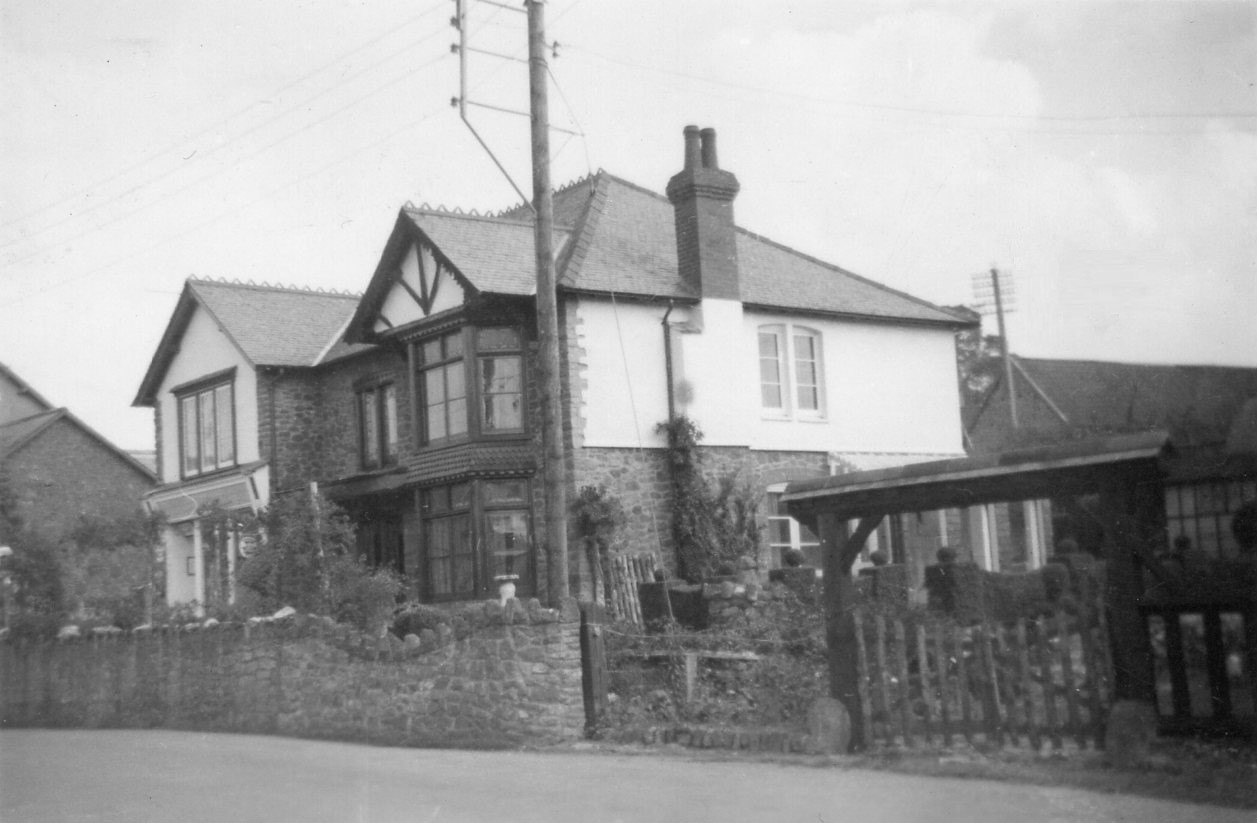
\includegraphics[width=1\textwidth]{figures/HillHeadHouse1960}
     \caption{A view of Hill Head House in the early 1970s}
     \label{fig:HHH1960}
\end{figure}

There is a certain satisfaction to be derived from having a \quotemark{good turn out}, and everyone, including the children, entered into the operation with gusto. We also had two kind ladies to help us, Miss Bates who had been assisting in the Post Office, and Cousin Kathie, who devotedly performed many thankless tasks for us in our absence. One of the disadvantages, which soon became apparent, was that it was impossible to close the shop while we were working as customers were continually coming and going, collecting pensions, or buying one 2 1/2d stamp - a never-failing source of astonishment to me but apparently a popular village pastime. I was amazed when one customer, a woman, came up to the Post Office three separate times in one day in order to buy a stamp. Later on, when I came to know the business better from my side of the counter, I ceased to be amazed at anything, but this was yet to come. At that time we were very eager to put a respectable face on things, but as work progressed we soon discovered that the slightest attempt to move anything from some of the shelves brought down choking clouds of dust - not exactly conducive to good customer relations!

We tackled the top shelves first as they looked fairly straightforward, being filled with piles of fairly large boxes rather than many small articles. It turned out that the boxes contained literally dozens of pairs of hobnailed boots - a standard form of footwear among farm labourers and formerly a good steady selling line. From the state of the boxes and from the handwritten prices in my father-in-law's writing it was obvious that they had been there for at least thirty years. I was puzzled by the algebraic symbols which appeared on the boxes and were repeated in pencilled writing under the insteps of the boots. Such combinations as \textit{lty}, \textit{xy}, \textit{opi} recurred with mystifying frequency but the explanation was quite simple. The letters were code for the cost price of the footwear, and the code, which apparently everyone in the family knew as well as their own names, was based on the extraordinary word DOLPHINET - D was 1, 0 - 2, L - 3 and so forth. 10, 11 and 12 were represented by x y z, hence the preponderance of these popular mathematical letters as 10/11 was a usual price for the older pairs. Another combination which I came to know well was \textit{lty} - 39/11. Kathie informs me that she became so familiar with the code in her years of running the Roadwater business that she could add up columns of the code letters as readily as figures. As the boots were so heavy to move, and both William and Ada were getting older, it seemed that as the years went by they had more or less forgotten what was in the boxes and under pressure from travellers ordered fresh stock which was put up on the top of the old.

As the customers had gradually been drifting away over the years, particularly after William's death, sales became less frequent and the boots piled up higher and higher towards the ceiling. Removing them all was a major task - I challenge any normal healthy housewife to carry more than four pairs of heavy nailed boots at once, even fewer if they are size tens and elevens! To the uninitiated (as I was) it should be explained that there are several sorts of	nail boots, light, medium and heavy and there are numerous variations of toe-cap and tongue. The problem was what to do with them all? Fortunately we had several outbuildings and after a certain amount of trial and error we eventually got the boots out of the shop and arranged them all in a building which we always refer to as the \quotemark{Toc H}. The children were of absolutely invaluable assistance in removing the boots from the boxes and carting wheelbarrow loads of perishing cardboard and rubbish up into the garden to be burnt. Altogether we counted about seventy-five pairs - and this in a small village shop! Throughout this operation it became obvious that we would have to have a sale of some sort. Though previously	we had had virtually no experience of the business - indeed had never been allowed to help - it turned out that I had quite a business flair where this sort of thing was concerned. A month or two more elapsed before we were sufficiently well organised to have a proper sale, but once the idea was established in our minds it was a great help in working out how and where to store the outdated stock.

Meanwhile Kathie and Miss Bates were doing their bit behind the Post Office counter, and soon they too were raising dust, throwing away old envelopes, or pulling out old telegram forms and envelopes to add to the rubbish heap. More and more boxes of old shoes were being discovered - children's boots and shoes going back to the early years of the century, ladles’ shoes of the 1920s, obsolete football boots, goloshes, even dancing pumps and leather gaiters. At this time the Automobile Association men still used to ride around on motor cycle combinations and they were the only customers who still used gaiters. The patrolmen used to come from miles around to buy them from us, and staunchly maintained that they were the best possible gear for keeping their legs and ankles warm and dry.

One brave soul started to explore the space under the large shop window. Apart from large quantities of cobwebs, and a generous supply of thirty year old cardboard boxes, it gave forth numerous bicycle accessories including a pair of handlebars, a couple of mudguards and a splendid carbide lamp. The children were highly delighted to find some toddlers straps made of solid leather with nice little metal bells on them - although long past the age of wearing such things my seven-year-old refused to take them off for days.

Of course, there were quite large quantities of stock which were fit for nothing and had to be thrown away. Torch batteries for example, out-of-date films, several venerable toothbrushes, and a strange substance called \quotemark{Amovon} Foot Paste. I wondered why there seemed to be so many tins of this commodity on every shelf, looking strangely out of place with its grotesque little illustration of a 1920s type sporting man wearing a huge cap. Apparently, during the bad years of the 1930s an unscrupulous \quotemark{traveller} desperate for trade, had deliberately falsified a reluctant order for one dozen boxes of this medicament to twelve dozen. Too busy or too unwilling perhaps to protest, William had retained the goods and there it was after thirty years.

The supply of shoe laces was also fruitful - some of them very broad and floppy, had been in fashion in the 1930s and by 1967, funnily enough, were once more being worn. To my shame I confess I threw the laces out for the dustman, but later discovered that my prudent preserver, alias Glyn, had saved them. This was a recurring performance, but I am pleased to say that I have now learnt more civilised ways and hoard in the best Court tradition.

What else did we achieve in that first mad rush of enthusiasm? A higher standard of cleanliness certainly, for as work progressed the Parkinson's law of spring cleaning started to come into effect, in other words as fast as we succeeded in scrubbing and cleaning one part, we realised how dirty was the part next to it. Fortunately, or unfortunately according to how you view the matter, Whit Monday was an official closing day so that we were able to make a thoroughly good job of exhausting ourselves. We even managed to splash some paint on the ceiling and walls. The more we progressed, the more it became obvious that we would have to write off a large amount of the stock and sell it for whatever it would fetch. So on the following day, with the children helping, we made a start by putting out quite a few of the old shoes at give-away prices, The children entered wholeheartedly in the sale idea and hid themselves behind the shop curtain in order to watch the proceedings. Tuesday is a busy day in the Post Office as the Family Allowances are given out, and there is always bound to be a steady flow of mothers and babies coming into the shop. As the previous day had been a Bank Holiday there were also a few pensioners as well. There was great excitement and loud stage whispers could be heard:

\begin{quote}
\quotemark{Sh! There's someone coming in!} (Giggle, giggle, fidget, heavy breathing) \\
\quotemark{She's looking at the shoes. She's buying them – quick come and look}
\end{quote}

etc. and so forth. Unfortunately this keenness had worn off by about ten o-clock in the morning! The word soon got around the village and people began to pop in and disappear again very quickly in order to tell their relations the good news about our bargains.

For a few weeks the children continued to enter into this new game with tremendous enthusiasm, becoming very excited, every time we succeeded in selling something. For a while, we kept a few sweets, and nothing would satisfy them but to have a small stall of their own in the shop. The youngest child carried this enthusiasm a little too far, as she felt so disappointed if no one bought anything that without telling anyone, she locked the door of the shop. When the customers, mostly friendly village ladies, found they could not get out they were held to ransom and forced to buy something. At this point parents intervened and hastily unlocked the door before losing their customers for good!

On many other occasions the children came in very useful, particularly in the later stages when we could not afford paid help, as they would guard the shop and call us if anyone came in. My eldest daughter must have done most of her O-level revision with the door into the shop partly open, and often interrupted her studies to sell a greetings card or a pair of bootlaces Though not likely to produce a certificate at the end, I feel it was education of a different sort. In fact the children often used to do small jobs about the shop which took a great deal of time and patience, and even when quite young, my eldest daughter had become accustomed to helping Ada to sort out the birthday and greetings cards. She became very possessive about them and if it had not been for her assistance we should never have managed to keep the cards tidy. Another job which the children never minded doing was sorting out the miniature cars. These used to live in a special stand under a pilfer proof cover. Unfortunately not only was it pilfer proof, it was also owner proof and occasionally the whole set of cars, numbered from one to seventy-five, would fall out while I was struggling with the cover on to the floor. Replacing them all took hours and it seemed rather a lot of work in order to make the modest sixpence profit on each car. As with all small items of trade one needs a fast sale and quick turnover to make it worthwhile selling them.
	
The children could often be induced to do little helpful jobs if I paid them a small wage, and the rate fixed for Joy, who was ten at the time, was sixpence an hour. After one enthusiastic week's work during the school holidays she managed to earn one pound - perhaps it was as well that no youth employment officer was on the scene to work out how many hours of work she had put in per day.

Over the next few months there was a great deal of rushing to and fro between Ilfracombe and Washford, and we wore out a good many tyres as we continually crossed and recrossed the lonely hills of Exmoor. Friday night was rather a headache, as Glyn had inherited willy-nilly his mother's responsibility for the Post Office and therefore, every week on Friday night the accounts had to be balanced up. The G.P.O. is a singularly bad employer in this respect. Our cousin, also a village postmistress, was completely flooded out in 1961 (to name but one occasion) by the nameless stream. Although there were three feet of sludgy water in her living room and Corn Flakes and postal orders floating around it it, she was not allowed to close the office. Instead of being allowed to get on uninterruptedly with the task of cleaning and drying her ruined home, she was obliged to hire the Village Hall (at her own expense of course) and conduct operations there. As a special concession in view of the floods, she was allowed to close in the afternoons. This happened on several occasions and certain articles of family furniture have permanent red shadows in their crevices - relics of floods in Grandfather's day. One hopes that the works undertaken by the Water Board will spare the inhabitants of Roadwater such misery in future.

Fortunately Glyn had had plenty of experience in counting rows of stamps, checking postal deposits and withdrawals, postal orders, pensions and so forth as it was the only department of the family business for which his mother considered that his University education had fitted him. Towards the end of her life I never ceased to be amazed that a woman of her age could add up long columns of figures with such effortless ease, but as my talents lie in other directions I was always only too pleased to leave this tedious task to them, and therefore I was not much help on Fridays. After Ada's death it meant that Glyn had to rush out of school on Friday afternoon at four o-clock and drive straight to Washford, where the accounts frequently would not balance. It then took quite a lot of the night and half of Saturday to get them right. Quite often the whole family went for the weekend but as anyone who has had two houses on their hands for any length of time will know, it is not exactly a picnic moving at regular intervals from one to the other with four children in tow, let alone having to count the stamps as soon as you arrive. We were in any case already leading a very full and busy life in Ilfracombe with frequent weekend engagements. The children were at school and naturally had all their friends and interests there, and Glyn was constantly working for his church and the Liberals, all of which was quite enough without inheriting a post office as well. Most of our social life was tied up with Liberal fairs, dances and suppers with Jeremy Thorpe, not to mention the regular bouts of canvassing and committee meetings, and we were reluctant to abandon all this happy activity. This conflict continued right up to the last day that we lived in North Devon. As the months went by it became increasingly obvious that we had loaded ourselves with an intolerable burden. Two houses to maintain with only a little money coming in to keep them going, two cars and the children - we could not possibly afford to continue without taking some decision. But by this time it was too late to do the sensible thing and sell the property. The voice of reason was very insistent that to sell was the only reasonable course of action. Unfortunately there were two major obstacles to this - neither based on logic or good sense, firstly, Glyn had promised his Mother that he would keep the house that his Father had built (he wanted to anyway) and secondly, we had by this time become hopelessly optimistic about all sorts of exciting projects for the shop which if fulfilled were going to change our destiny. Children with a new toy would be an apt, if hackneyed, metaphor. Dreaming of a new wave of prosperity our fantasies knew no bounds, and we eagerly embraced and swallowed success stories of village stores expanding into small empires. At one point, I remember, we mapped out the orchard as a park for our fleet of delivery vans. There was literally no limit to the variety of stock which we thought we might sell, and certainly no bounds to our enthusiasm at that time, how thankful I am that the orchard project never came to anything! The sight of the grass overshadowed with apple-blossom is worth far more than a quarter of an acre of tarmacadam, while the early morning song of blackbirds and thrushes too is infinitely precious. I can even learn to love the cooing of the rapacious pigeons in the copse at the top of the garden when I think that had our wild imaginings been realised we should have been completely hemmed in by the sound of the internal combustion engine. A narrow escape indeed.